\section{A Search for \ttbar\ Resonances}

\subsection{Strategy}

\begin{frame}
    \frametitle{Strategy I}
\begin{columns}
\column{.4\textwidth}
\begin{itemize}
    \item \ttbar\ collision events are selected in the single lepton
        (lepton plus jets) decay channel.
    \item Leptons created through electroweak processes at the LHC
        $\to$ backgrounds are reduced
    \item Dilepton decay channel
\begin{itemize}
        \item Small branching fraction,
        \item Two neutrinos: \mtt\ cannot be fully reconstructed.
\end{itemize}
\end{itemize}
\column{.6\textwidth}
\centering
\begin{tabular}{l|r}
    \hline
    Process                         & $\sigma$ (pb)      \\
    \hline
    Multijet                        & $72 \times 10^9$   \\
    \wjets\ ($W \to \ell \nu_\ell$) & $34 \times 10^3$   \\
    \zjets\ ($Z \to \ell\ell$)      & $2.9 \times 10^3$  \\
    \ttbar\ ($>= 1\ell$)            & 110                \\
    Single top ($>= 1\ell$)         & 49                 \\
    $WW,WZ,ZZ$ ($>= 1\ell$)         & 17                 \\
    \hline
    \hline
\end{tabular}
\end{columns}
\end{frame}

\begin{frame}[label=strat2]
    \frametitle{Strategy II}
    \centering
\begin{itemize}
    \item Two reconstruction strategies for the hadronically-decaying
        top quark
        \begin{itemize}
        \item ``Boosted'': all decay products contained in one jet
            with $R=1.0$
        \item ``Resolved'': decay products reconstructed as three
            $R=0.4$ jets
        \end{itemize}
    \item \mtt\ is reconstructed for each event.
    \item Spectra from the data and SM predictions are compared to
        assess the validity of two models which predict resonant
        production:
    \begin{itemize}
        \item \hlink{extradims}{Randall-Sundrum Warped Extra
            Dimension} (heavy gluon, $\kkg$)
        \item \hlink{topcolor}{Top Assisted Technicolor} (heavy
    $Z$-like boson, $\zp$)
    \end{itemize}
\end{itemize}
\includegraphics[height=3cm]{ttbarevent.png}
\end{frame}

\subsection{Data and MC Samples}

\begin{frame}
    \frametitle{Data and Monte Carlo Samples}
\begin{itemize}
    \item $\int \mathcal{L}~dt = 14.3~{\rm fb}^{-1}$ of $\sqrts =
        8$~TeV proton-proton collisions are analyzed.
    \item Standard Model predictions are derived using Monte Carlo
        techniques for most background processes.
    \item The dominant non-\ttbar\ background, \wjets, is modeled
        using MC, but the prediction is corrected using collision
        data.
    \item Backgrounds with non-prompt leptons are derived entirely
        using collision events.
    \item The production of the signal RS Kaluza-Klein gluon and Topcolor $Z^\prime$
        boson benchmarks are simulated using Monte Carlo.
\end{itemize}
\end{frame}

\subsection{Event Selection}

\subsubsection{Common Selection}

\begin{frame}
    \frametitle{Common Selection}
\begin{figure}
\centering
\includegraphics[height=2.5cm]{ttbarevent.png}
\end{figure}
\vfill
A selection is applied to collision events to reduce the background
from non-\ttbar\ production processes:
\begin{itemize}
    %% TODO
    %% neutrino constraint backup
    \item Exactly one high-$p_T$ ($> 25$~GeV) electron or muon
        which passes tight quality and isolation cuts
    \item $\met > 20$~GeV (30~GeV) in the muon (electron) channel
    \item
        %% TODO
        %% $\mt = \sqrt{2 p_T^{\ell} \met (1-\cos \Delta \phi)}$
        $\met + \mt > 60$~GeV ($\mt > 30$~GeV) in the muon (electron)
        channel.
    \item The neutrino $p_z$ is solved for using the $W$ boson mass as
        a constraint.
\end{itemize}
\end{frame}

\begin{frame}
    \frametitle{Common Selection}
\begin{figure}
\centering
\includegraphics[width=.5\textwidth]{QCDTriangularCut.png}
\includegraphics[width=.5\textwidth]{ttTriangularCut.png}
\end{figure}
\vfill
\centering
Illustration of the rejection of QCD backgrounds with the $\met$ and
\mt\ requirements in the muon channel
%% (PhD thesis of Bálint Radics)
\end{frame}

\subsubsection{Boosted Selection}

\begin{frame}[label=boostedsel]
    \frametitle{Boosted Selection}
\begin{figure}
\centering
\includegraphics[height=2.5cm]{boostedevent.png}
\end{figure}
\vfill
\begin{itemize}
    \item The highest-$p_T$ \smallr\ jet with $\dr(\ell,\ jet) < 1.5$
        identified as the $b$ quark jet on the leptonic side

    \item The \hlink{trimming}{trimmed} \larger\ jet must satisfy
    \begin{itemize}
        \item $p_T > 300$~GeV, $m > 100$~GeV, $\dsplit > 40$~GeV,
        \item $\dr > 1.5$ from the selected \smallr\ jet.
            %% $\Delta \phi > 2.3$ from lepton.
    \end{itemize}

    \item One \smallr\ jet must be \hlink{btagging}{$b$-tagged}.

    \item \mtt\ = mass of four-momentum sum of the lepton, neutrino,
        selected \smallr\ jet, and selected \larger\ jet.
\end{itemize}
\end{frame}

\begin{frame}
    \frametitle{Boosted Selection}
\begin{figure}
\centering
\includegraphics[width=.5\textwidth]{trimmedtopjetmass.pdf}
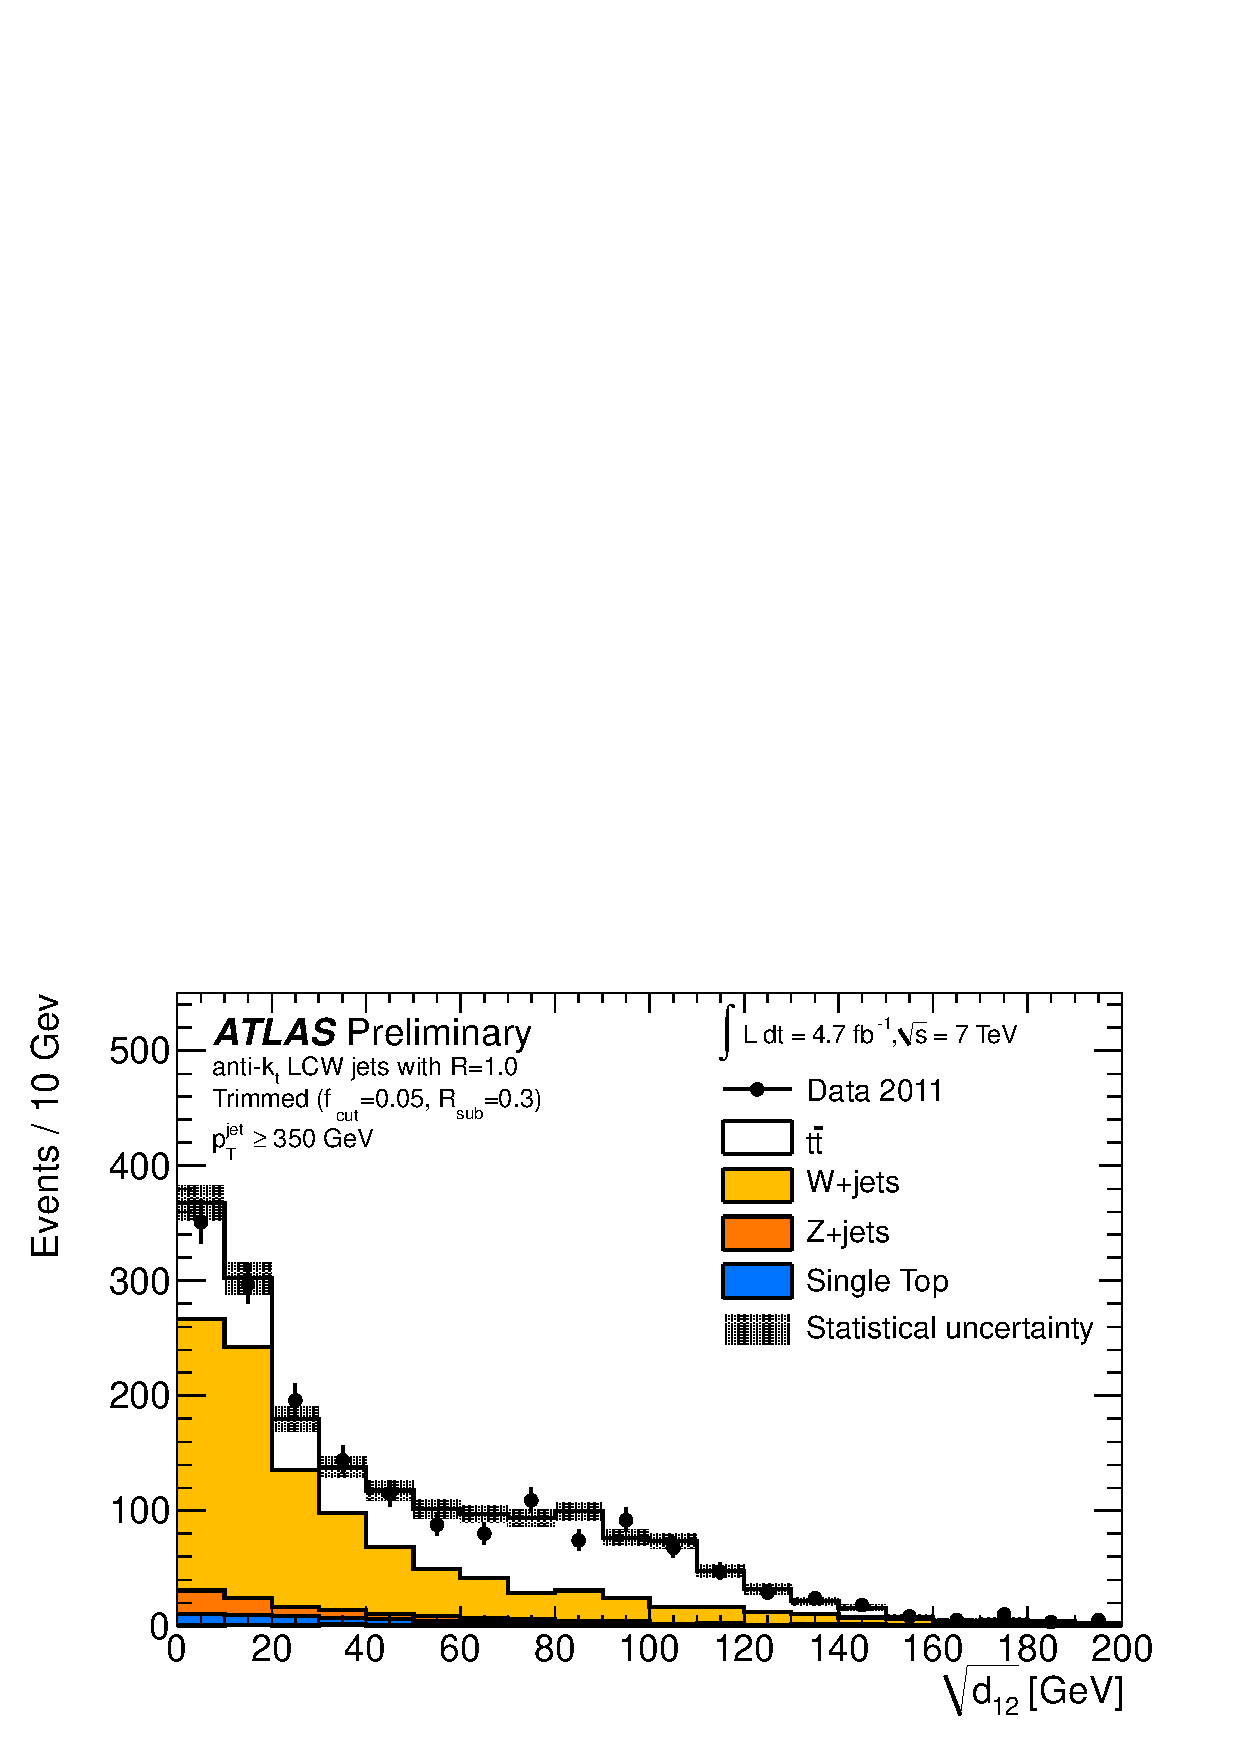
\includegraphics[width=.5\textwidth]{trimmedtopjetd12.pdf}
\end{figure}
\vfill
\centering
Illustration of the rejection of non-\ttbar\ backgrounds with the
hadronic top jet $m > 100$~GeV and $\dsplit > 40$~GeV requirements in
the boosted selection
\end{frame}

\subsubsection{Resolved Selection}

\begin{frame}
    \frametitle{Resolved Selection}
\begin{figure}
\centering
\includegraphics[height=2.5cm]{resolvedevent.png}
\end{figure}
\vfill
\begin{itemize}
    \item Fail boosted selection
    \item There must be four \smallr\ jets with $p_T > 25$~GeV.
    \item If there are excess \smallr\ jets in the event, a
        likelihood function is used to identify those from the \ttbar\
        pair.
    %% \item Only three are required if one \smallr\ jet has a mass
        %% $m > 40$~GeV.
    \item One \smallr\ jet must be \hlink{btagging}{$b$-tagged}.
    \item \mtt\ = mass of four-momentum sum of lepton, neutrino, and
        selected jets.
\end{itemize}
\end{frame}

\subsubsection{Candidate Event}
\begin{frame}
\centering
\frametitle{Candidate Event}
\begin{figure}
    \includegraphics[height=6cm]{evtdisplay.png}
\end{figure}
\end{frame}


\subsubsection{Selection Efficiency}
\begin{frame}
    \frametitle{Selection Efficiency}
\centering
The combined selection efficiency of \ttbar\ events
\begin{figure}
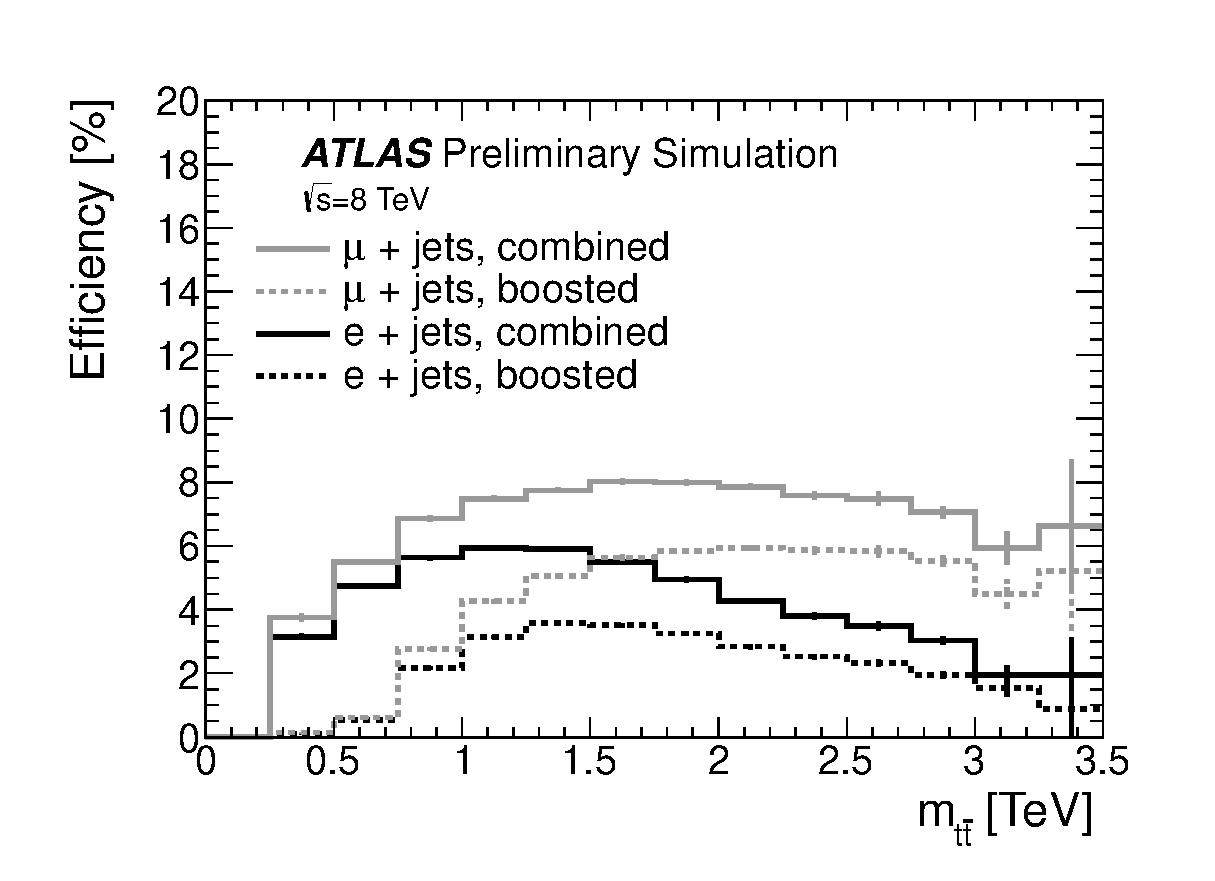
\includegraphics[width=.75\textwidth]{selectionefficiency.eps}
\end{figure}
\end{frame}

\subsubsection{\mtt\ Reconstruction}
\begin{frame}
\frametitle{\mtt\ Reconstruction}
\begin{columns}
\column{.5\textwidth}
\centering
The reconstructed \mtt\ spectrum for various signal benchmarks in the
boosted channel
\begin{figure}
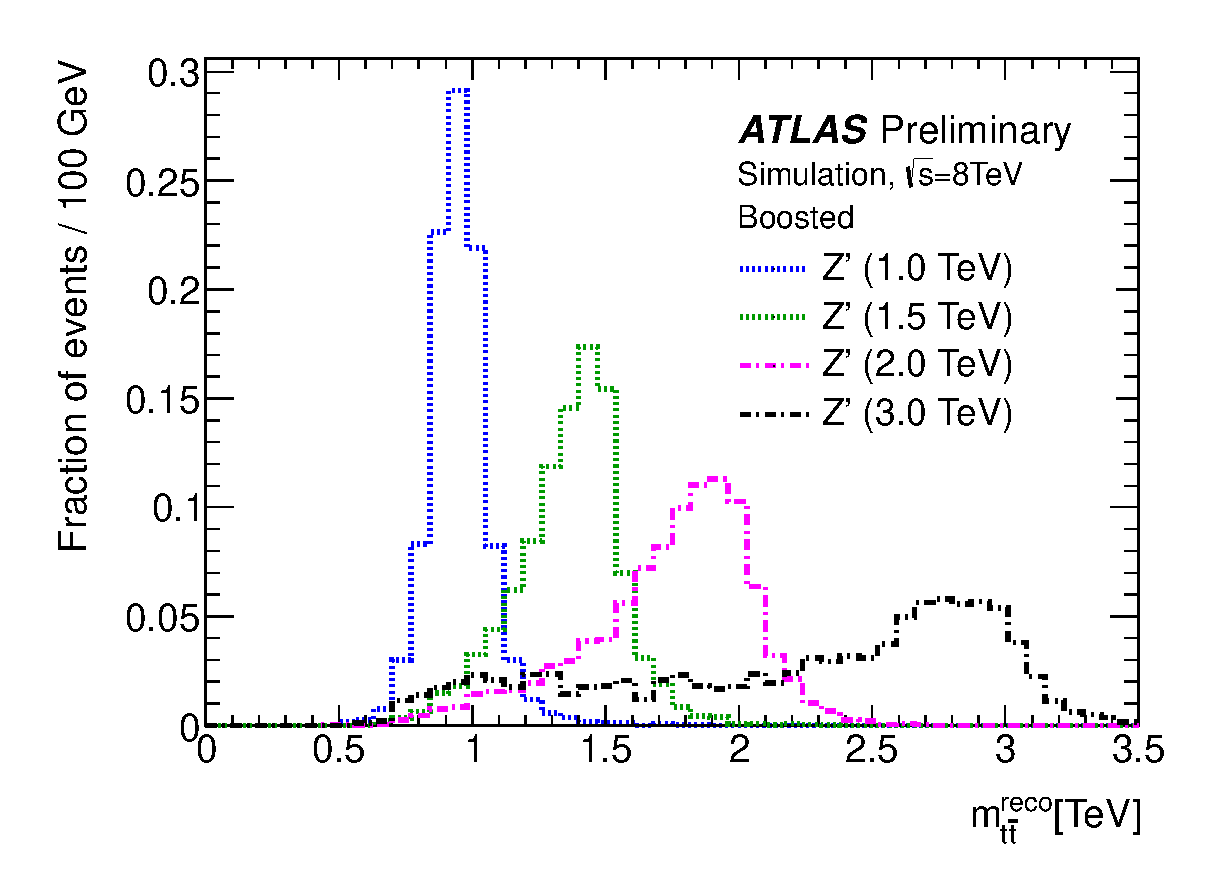
\includegraphics[width=\textwidth]{zpmttboosted.eps}
\end{figure}
\column{.5\textwidth}
\centering
The \mtt\ resolution for various signal benchmarks in the boosted
channel
\begin{figure}
\includegraphics[width=\textwidth]{zpmttresoboosted.eps}
\end{figure}
\end{columns}
\end{frame}

%% TODO

\begin{comment}
\subsection{Data-Driven Backgrounds}
\begin{frame}
    \frametitle{Data-Driven Backgrounds}
\begin{itemize}
    %% TODO
    \item Some SM backgrounds are derived using collision data: \wjets\
        and backgrounds containing non-prompt leptons (multijet).
    \item The normalization and heavy flavor content of the \wjets\
        background is corrected for by using the charge-assymmetry of
        $W^+$ and $W^-$ events at the LHC\@.
        \begin{itemize}
        \item Since the LHC is a $pp$ collider, $W^+$ events have a
            higer cross section than $W^-$ events.
        \item The relative fraction of $W^\pm$ events is significantly better
            understood than the total \wjets\ cross section.
        \end{itemize}
    \item The multijet background is estimated by measuring the
        false-identification rate of non-prompt leptons in an enriched
        control region and the efficiency of prompt leptons from
        \ttbar\ MC events.
\end{itemize}
\end{frame}
\end{comment}

\subsection{Systematic Uncertainties}

\begin{frame}[label=systematics]
    \frametitle{Systematic Uncertainties}
    \begin{itemize}
        \item The effects of several systematic uncertainties on the
            final \mtt\ spectrum are assessed.
        \item The most important sources of uncertainty are
        \begin{itemize}
            \item LHC luminosity (3\%),
            \item \ttbar\ production cross section (9\%),
            \item proton structure (6\%),
            \item \hlink{boostedjes}{energy calibration of \larger\
                jets} (16\%),
            \item parton shower model (4\%),
            \item efficiency of tagging $b$ jets (3\%).
            %% TODO
            %% add table in backup
            %% Sudakov
        \end{itemize}
    \end{itemize}
\end{frame}

\subsection{Data and Background \mtt\ Comparison}

\begin{frame}
\frametitle{Data and Background \mtt\ Comparison}
    \centering
The agreement between the data and SM prediction is assessed using the
reconstructed \mtt\ spectrum.
\begin{figure}
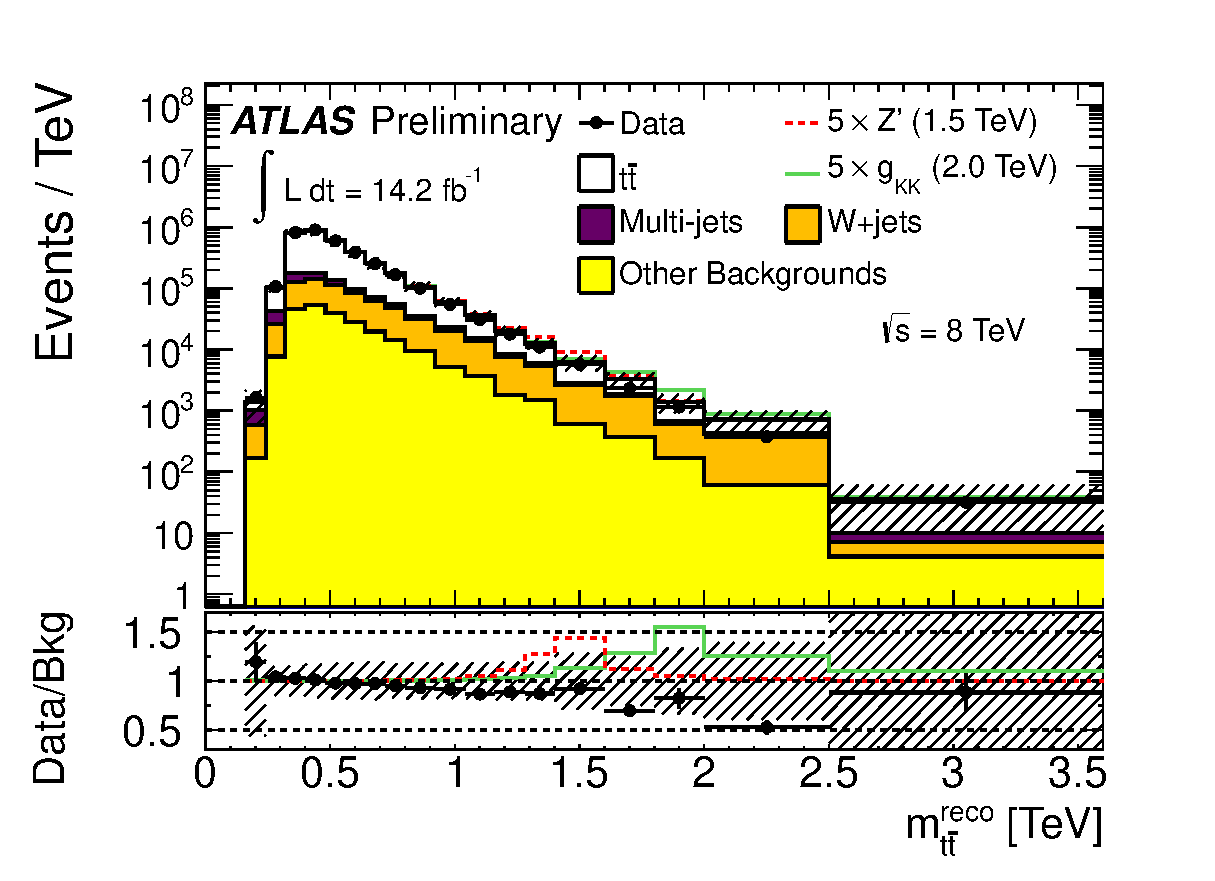
\includegraphics[height=5.5cm]{combinedmtt.eps}
\end{figure}
\end{frame}


\subsection{Results}


\begin{frame}
    \frametitle{Statistical Methods}
\begin{itemize}
    \item In the absence of significant deviations from the SM
        prediction, upper limits on the cross section times branching
        ratio for the signal benchmarks are set.
    \item The likelihood $L_\nu$ for a resonance mass $\nu$ with cross
        section $\sigma_\nu$ is the product of the Poisson
        probabilities of the data measurement given an expectation of
        the signal plus background in each bin:

\begin{equation*}
    L_\nu(D | s_\nu, b) = \prod_{{\rm all\ bins}\ i}
    \frac{e^{-(s_{\nu,i} + b_i)} {(s_{\nu,i} + b_i)}^{D_i}}
    {D_i!}.
\end{equation*}

\noindent $D_i$, $b_i$, $s_{\nu,i}$ are the number of data events,
total predicted background yield, and signal yield in bin $i$,
respectively.

\end{itemize}
\end{frame}

\begin{frame}[b]
    \frametitle{Results}
    \centering
Upper cross section limits at 95\% credibility for the two signal
benchmarks
\vspace{0.5cm}
\begin{columns}
    \column{.5\textwidth}
    \centering
    Kaluza-Klein gluon ($\kkg$) in RS models excluded for
    $0.5~{\rm TeV} < m_{\kkg} < 2.0$~TeV
\begin{figure}
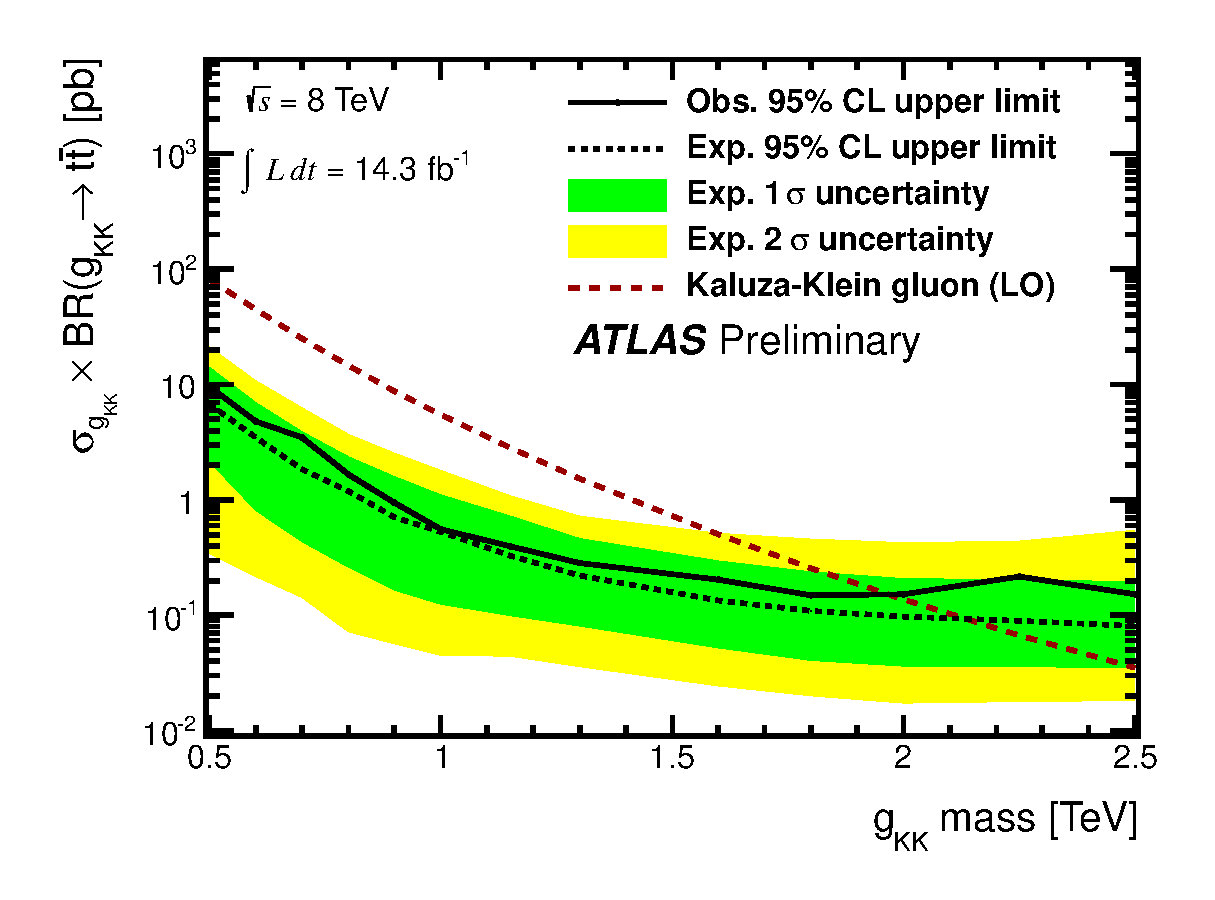
\includegraphics[width=\textwidth]{kkglimits.eps}
\end{figure}
    \column{.5\textwidth}
    \centering
    Leptophobic $Z^\prime$ boson in Topcolor Assisted Technicolor
    excluded for $0.5~{\rm TeV} < m_{\zp} < 1.8$~TeV
\begin{figure}
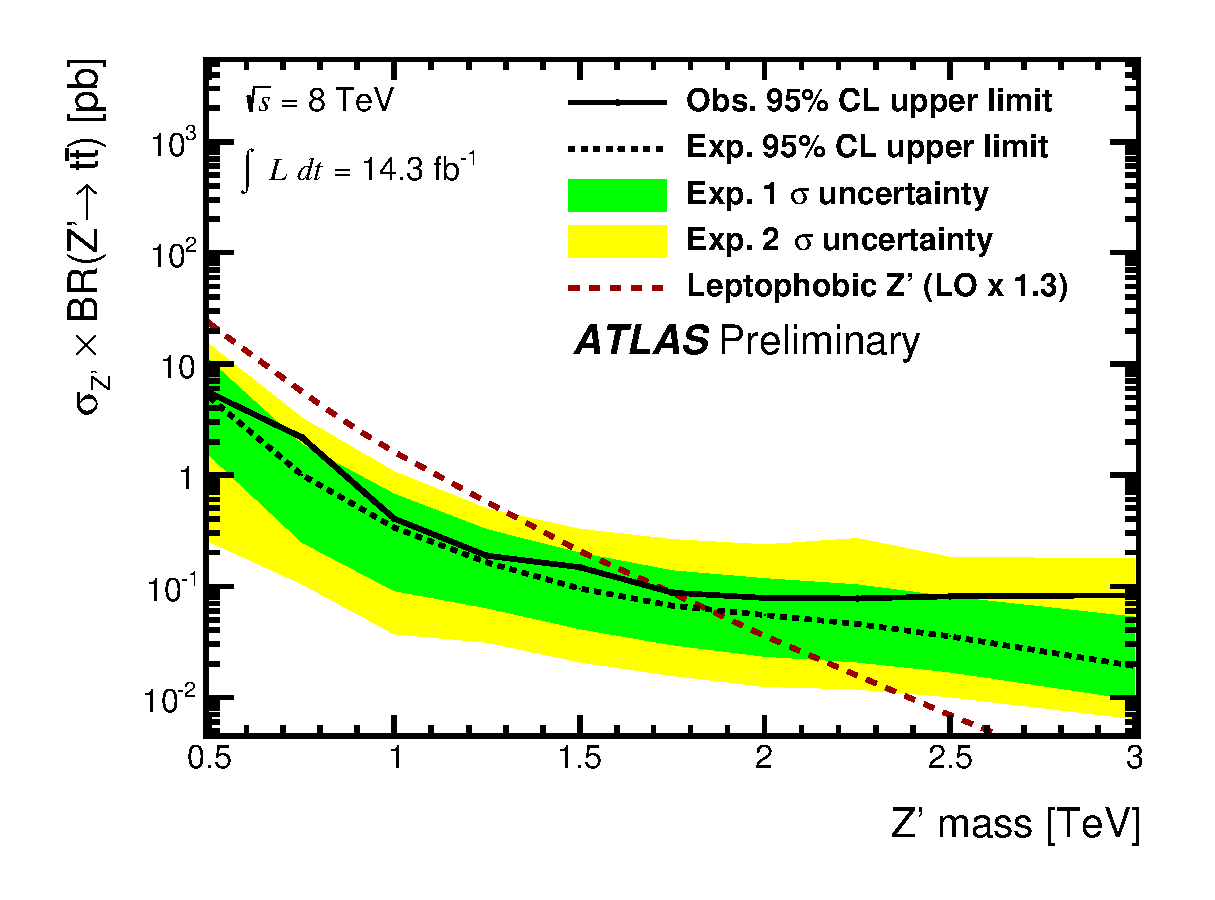
\includegraphics[width=\textwidth]{zplimits.eps}
\end{figure}
\end{columns}
\end{frame}
